\documentclass{article}
\usepackage[utf8]{inputenc}
\usepackage{indentfirst}
\usepackage{graphicx}
\usepackage[english]{babel}
\usepackage{biblatex}
\addbibresource{biblio.bib}

\providecommand{\keywords}[1]
{
  \small	
  \textbf{\textit{Keywords---}} #1
}

\title{Are You Warm-Blooded? The Effect of Hometown Climate on NFL Running Backs' Performance in Freezing Temperatures}
\author{Lydia Margolien}
\date{December 9, 2022}

\begin{document}

\maketitle

\section{Abstract}
\noindent This paper seeks to analyze the effect of an individual's lifetime climate on their athletic performance in freezing temperatures. Colloquial discussions of being "cold" or "warm" blooded indicate that many individuals feel as though they are better acclimated to one climate or another. For most individuals, this preference usually manifests in general comfort levels and preferred locale of residence. For athletes, however, preferred climate may seriously impact a player's performance in certain temperatures. This paper examines NFL running backs' performance in freezing temperatures and if the climate in which they were raised affects their performance. Applications of this research could be used for coaching, training, and fantasy football insights. 

\keywords{NFL, sports analytics, game conditions, lifetime climate, running backs}


\section{Introduction}

\noindent Many Americans have an affinity for the climate of where they grew up. Northerners hesitate to move to the South because of the oppressively hot summers and lack of true cold weather in the winter. Southerners may feel as though they are "warm blooded" and will be unable to handle the Northern winter cold. Effects of preferred climate on travel and migration patterns as well as athletic performance are often subject of casual conversation and investigation. While many journalistic pieces have speculated on effect of weather on play performance, few academics have delved into this area of research \cite{pracsport} \cite{injrate}. Sports journalists will speculate on a team's performance in a cold weather game, for instance, based on where the team's home field is (for example, the Buffalo Bills are certainly better acclimated to playing in cold and snowy games than the Miami Dolphins \cite{5worst}. But what about the effect of weather on individual players? \\\\

\noindent This paper seeks to answer how a player's hometown climate (lifetime climate) affects their performance. That is, are people truly better acclimated to weather similar to where they grew up? This study specifically analyzes NFL running backs' performance (by examining yards per carry, referred to as YPC) in games played in freezing temperatures (32 degrees Fahrenheit or below). Lifetime climate has been determined by looking at the average temperatures of a players' hometown and where they played college football. Players that grew up in areas \textit{and} played college football in locations with January and February average temperatures above 50 degrees Fahrenheit were examined against players whose hometowns and college towns did not fit this standard. This paper seeks to answer if there is a significant difference in performance in freezing temperatures between people with lifetime colder climates than those who usually did not experience freezing weather. \\\\

\noindent Several studies in the field of sports medicine have examined how cold affects athletic performance \cite{coolperformance} \cite{outincold} \cite{pracsport}. Studies have shown that the maximum contractile power of muscle decreases as temperature decreases. Additionally, most sport research has focused on performance in endurance sport or cold weather sports such as cross-country skiing and ultra marathons and triathlons \cite{pracsport}. While professional football players certainly train extensively and have elite cardiovascular fitness, the actual playing of a football game is not an endurance sport. Unlike soccer, basketball, or ice hockey, players perform in short bursts of exercise, such as sprinting or tackles that last less than 10 to 15 seconds at a time. In between plays, there is ample rest time for athletes on the field. In some aspects, cold may benefit player performance. In order to keep body temperatures adequately warm, the brain releases norepinephrine to keep our bodies shivering, to increase blood flow, and raise blood pressure \cite{outincold}. Slightly raised blood pressure may increase sport performance; however the norepinephrine keeps blood circulating closer to the core, which may lead to decreased blood flow in the extremities. For a sport like football which relies on quick footwork and intense eye-hand coordination, the decreased blood flow to the extremities would hinder fine motor skills that would be necessary for fast maneuvering on the field to get around defenders, and for catching passes (as well as throwing passes for quarterbacks). \\\\

\noindent The cold may also impact athletes in not just physical ways. Psychology is extremely important to player performance, with some athletes and coaches going so far to say that is most of athletic performance. Pain tolerance in sport is important to the athlete's psychology \cite{pain}. Of course, professional athletes are no stranger to pushing through pain during performance. However, climate conditions are a unique kind of pain that requires a kind of adaptation that may be very unfamiliar to a player who has not experienced that climate before. Climate has an overall effect on mood as well that would require a different kind of psychological processing compared to persevering through calf pain that disappears when weight is removed from the leg, for instance. Researchers have found that hometown climate does affect individuals' predisposition to experiencing seasonal affect disorder, indicating that there is a connection between hometown climate and some aspect of climate stimulus processing \cite{hawaii}. \\\\

\noindent Performances in freezing temperatures were examined because these temperatures are unique to certain parts of the country. The vast majority of locales in the continuous United States experience very warm temperatures and heat waves throughout a summer, even if the average summer temperature is lower than in the South. However, some Americans live in locations that may go years without snow or high temperatures of freezing or below. This means that there almost all Americans will experience very hot weather at some point, but not all Americans will be exposed to freezing temperatures. Additionally, certain states that experience freezing and snowy temperatures may be so unprepared for such weather that when it does snow or ice, the state shuts down. For example, central North Carolina is north enough that it will usually experience snowy and icy conditions once a year or so, however its road and utilities infrastructure (as well as individual residents) is unequipped for these weather events. Even in an inch of snowfall can result in road closures, school cancellations, and many traffic accidents and power outages \cite{ncsnow}. This means that players from locations that see winter but not often may have never had to actually play or actually experience the cold weather because their schools and roads were closed which would result in game and practice cancellations. \\\\

\noindent There are several possible applications of the outcome of this study and sequential studies with similar designs. First, outcomes of this study could be used as a factor in a franchise's decision to cover their stadium with a dome. While there are other factors that go in to this decision, such as franchise budget and construction costs and how it would impact fan involvement (some fans are very against the idea of domes), doming could provide an advantage as teams are guaranteed to play at least half their games in mild weather. Retractable domes are specifically helpful because should a team decide to train for a cold-weather play off game, they could do so depending on their location. Academic research has not tackled studies involving game performance in domed stadiums compared to outdoor stadiums. Sports fans, specifically fantasy statisticians have run some studies on the advantages or disadvantages of playing under a dome. Historically, teams struggle with their season record when they first start playing in a dome. Quarterbacks perform better in their home domes, but visiting quarterbacks also do better when playing in another team's dome \cite{domeadv}. Domes importantly do not only shield from cold air temperatures; domes also protect against wind, glare from the sun, and can alter depth perception when tracking the ball. Fantasy statistician Keaton Denlay has found that while there is not a specific advantage for a team performance (although there is for quarterback performance), games played in domes, on average, are higher scoring than 96 percent of games played outdoors \cite{denlay}.  \\\\

\noindent Secondly, outcomes of this study could be used to inform NCAA football recruiting decisions. While players generally want to go where the best coaches are, for the very best high school players, they have many options to choose from. For high school recruits from warm climates, outcomes of this study could guide them to determining if it would help their potential NFL career and draft possibilities to choose a school with a cooler climate to gain exposure to new climates and outperform other college players. As youth sports gets more and more competitive in the United States, some wealthy and die-hard sports parents may even make the decision to move regionally or send their child to a certain boarding school in better chances of improving their playing career based on climate differences.  \\\\

\noindent Third, outcomes of this study could be used by franchise's to decide if they devote more of fewer resources to climate adaptation practices. Similar to the idea of doming their stadium, teams could decide if it would be worth it to invest in technology and facilities that would allow players extra time to practice in cold temperatures before an upcoming game. \\\\

\noindent Outcomes of this study can be used to enlighten casual conversation and fan conjecture about a team or player's performance in a cold game. Other studies as well could take from this experimental design and improve upon it or otherwise alter it to obtain different results. Researchers from other disciplines such as sports medicine, kinesiology, and economics could also use outcomes from this study. Medical research may benefit from long-term studies of cold adaptation in its relation to brown adipose tissue acclimation. Brown adipose tissue (BAT) is a certain kind of fat that helps mammals stay warm. BAT is found in higher proportions in infants than in adults but adults do have BAT in their bodies  as well \cite{bat}. Sports economists may also benefit from data analysis on weather patterns and game performance and in turn, game day spending. \\\\

\noindent Finally, with states starting to legalize sports gambling, studies analyzing performance in cold weather could be used in gambling analysis for both Vegas odds and fantasy football odds. Player odds could be enhanced with climate specific data. \\\\

\section{Data Description}
\noindent Games were selected from the 2017, 2018, and 2019 National Football League (NFL) season. To be considered in this study, games had to be played outdoors in below freezing temperatures for all four quarters. Temperatures per game were found from weather.gov for the day, time, and location of the stadium during game time. The 10 domed stadiums in the NFL were automatically excluded from the study. \\\\

\noindent Running backs' performance statistics were taken from nfl.com. While the running back data itself is not sampled randomly (these statistics take into account every play that a player made in a single game), the players were randomly selected in that all NFL teams play in cold temperatures essentially randomly. Players will have to play in cold temperatures no matter their lifetime climate as players do not play for professional teams based on where they are from. NFL season schedules are not generated randomly, however the conditions that need to be met during the schedule creation process are not influenced by climate patterns \cite{nfl}. Thus, there is an element of "chance" (that is, randomness) that may indicate when in the season one team may play another team located in a Northern climate that would be more likely to experience freezing temperatures in the later part of the season. \\\\

\noindent Yards per Carry (YPC) were used because this is the statistics that is most commonly used to evaluate running back performance as it specifically assesses how well a player can carry the ball. Running backs, as their name will indicate, specialize in rushing the ball, which means to run the ball down the field while avoiding and powering through the opposing team's defense. These players are usually powerful and athletic as they must be aerobically fit and strong. \\\\

\noindent While NFL quarterbacks are the most analyzed player in football, there are so few of them that using quarterbacks for this study would require data to be included from many more seasons. Not only are there fewer quarterbacks in the NFL (and usually only one quarterback plays per team per game), teams generally hold on to their quarterbacks for years at a time. Up to four running backs may see playing time for a team in any game, and they are more likely to be switched out in between and within seasons. With higher injury rates for running backs as well as a higher abundance of them, turnover is higher in the NFL leading to more data being available for this study. \\\\

\noindent NFL games were selected because they are the only American major sports league that plays a substantial amount of games outdoors in the winter. The Major League Baseball season ends at the end of October, barely after many cities have experienced their first frost. The NFL season plays through December and January when most locations experience their lowest winter temperatures. The PGA Tour (Professional Golf Association) will play almost year-round, however they choose warm weather locales in the autumn, winter, and early spring. The NBA exclusively plays indoors. Running statistics would have been difficult to analyze since the defined "professional leagues" usually refer to Olympic qualifiers and Olympic teams which often run in indoor tracks. \\\\

\noindent When athletic performance in extreme temperature conditions are discussed, the public's imagination usually focuses on popular sports such as football or baseball. Therefore, football is a great sport to analyze, especially considering that many of the popular football events (Thanksgiving Day games, playoff games, and the Superbowl) are played in winter. Fans will layer up to watch these games played in outdoors even in single-digit temperatures. As such, extreme (usually extremely cold) temperatures are a substantial part of the fan experience. For amateur players and local football fans, football is associated with cooling football temperatures as football is a fall season sport. For many individuals from the north and other climates with cold weather, this may lead to a feeling of superiority as these players and fan feel that their team is tougher for being able to handle and play well in these extremes. While extreme heat is also uncomfortable, humans can adjust to heat and survive. It is more difficult to survive on your own in colder temperatures as multiple layers of clothing and protection are necessary to protect against frostbite and dangerously low body temperatures. \\\\

\noindent Running backs' performance was selected out of convenience. While quarterback performance is intensely analyzed with many statistical metrics, only one quarterback per team usually plays in each game. Multiple running backs will play in a game; this allows for a smaller number of seasons to be examined. It was important to reduce the amount of seasons to eliminate possible other confounding factors. There are many possible confounding factors that may appear if data were taken from a wide range of seasons. The first is that the video and data analysis technology that the NFL uses to calculate their statistics has continued to improve over time. If quarterback performance was selected, it was possible data would had to have been collected across a ten year range, according to my initial data sweep. This would mean that the precision of technology from 2009 would be compared to the technology of 2019. Since video playback and data analytic technology rapidly changes over time, it would be best to control for the as much variation in data collection as possible. Secondly, it would take more time to collect data across different years. Data collection for any study should prioritize efficiency in data collection, and collecting data on quarterbacks would be unnecessarily time-intensive. If this study were to be continued by the NFL or another sports analytics group, time spent collecting data on quarterbacks would take more money. Since our goal is to simply measure player performance in cold, it does not necessarily matter if we examine quarterbacks or another football position, so one should prioritize for data collection efficiency. Third, changes in coaching and team management may impact player performance over time. For instance, many professional teams (in and outside of the NFL) as well as collegiate teams experience stretches of seasons where they perform very well or very poorly that were caused by changes to team leadership. While there certainly can be fluctuations in coaching management during the time period of this study (across 3 seasons), fluctuations are minimized. Fourth, there have been many innovations in heat and clothing technology over time. Athletic wear companies such as Nike, Adidas, and Under Armour, continually improve their thermal and athletic wear for warming or cooling purposes. As such, changes in NFL uniform and supply brands over time would also include changes in player technology and fashion trends. For instance, in different seasons it has been more or less fashionable for players to have their biceps exposed or to have some leg skin exposed between their socks and the uniform pants. Certain  layering pieces have certainly improved in quality over the past 10 years to keep players warmer in the game. As well, NFL teams have been adding heated benches to their stadiums to keep their players warm. \\\\ 


\noindent Additionally, good quarterbacks in the NFL are very rare. Since the position is so technically difficult and specialized, there are massive fluctuations in the skill of quarterbacks and backup quarterbacks. Each team will employ backup quarterbacks in a season, but their performance in even the most mild playing conditions significantly and regularly lags far behind the starting quarterback for a team. Thus, including backup quarterbacks would interfere with the normality of the data. While there is certainly variation in the quality and performance of running backs, there is less of an abrupt divide in skill between starting and back up players. There is more of a continuum in skill set between running backs on a team. \\\\

\noindent Yards per carry (YPC) is a statistic that considers the number of carries a player had in a game and the number of total yard gains the player made throughout the game, calculated by the formula:

\(T / C = YPC\)

where T = total yard gain in the game, where $T \in \mathbb{I}$ and C = number of carries, where $ C \in \mathbb{N}$. 

\noindent The yard gains and number of carries and corresponding YPC were calculated for each player and each game by nfl.com. The yard gain of each particular carry is not calculated. YPC is not a statistic specific to running backs. YPC will be calculated for quarterbacks, tight ends, wide receivers, and sometimes other offensive players as well. The running back position is usually more responsible for running the ball, that is "carrying" (which involves breaking through tackles and being a bigger player), whereas the wide receivers are more specialized in catching the ball. Since these positions all differ in their specialty, it is best to compare running back (RB) YPC compared to other RBs for consistency. \\\\

\noindent For each RB, information about their college and hometown was collected from nfl.com. From there, information about the average monthly temperature in each of their college and home towns was collected from weather.gov. As it is not uncommon for athletes to transfer colleges for athletic programs, several players had multiple college towns to consider. It was assumed for the purposes of this study that ever NFL player also played at least one season of high school football as it is extremely competitive to make it into the NFL. Therefore, it was also assumed that they were exposed to the climate of their high school locales. \\\\

\section{Methods}
\noindent Players who experienced a "warm" lifetime climate (their hometown and college town had average temperatures above 50 degrees Fahrenheit in January and February) were compared to players who did not meet this criteria. The "warm" lifetime climate distinction was strict- if a player lived most of their life in the south and played even just a year of college football in a cooler climate they were removed from the warm climate group. These groups were coded accordingly in the constructed R data frame. \\\\

\noindent Summary statistics for the mean and standard deviation were computed in R. \\\\ 

\noindent Table 1 
\begin{center}
\begin{tabular}{|c|c|c|}
\hline
Lifetime Climate Group & Mean & Standard Deviation \\
\hline
Warm & 3.956111 & 3.872995 \\ [1ex]
Cool & 4.17027 & 3.582431 \\ [1ex]
\hline

\end{tabular} 
\end{center}

\noindent  \\\\
\noindent A two sample Student's t-test to test for difference of means was used with a confidence level of 0.95. A t-test was used instead of a z-test because the population is just above 30 and the population standard deviation of running backs' performance in freezing games is unknown. The Student's t-test was published by WS Gosset in 1908. Over a century later, it is still one of the commonly used statistical methods for testing significant differences between two groups. \\\\

\noindent Before proceeding with the t-test, the normality assumption was tested with a histograms of the data for the warm and cold groups that showed a unimodal and approximately symmetrical distribution of the YPCs for the cold and warm weather groups. \\\\

\begin{figure}[htpb]
    \centering
    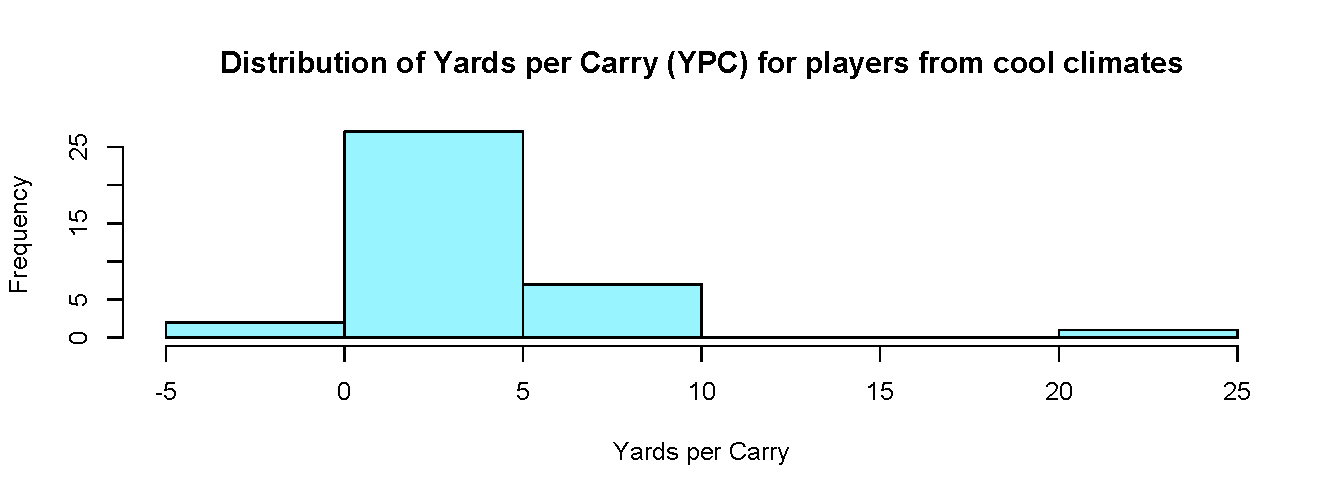
\includegraphics[width=0.8\textwidth]{histC.pdf}
    \caption{Histogram of YPCs for players from cool lifetime climates}
    \label{fig:tikzpgf}
\end{figure}

\begin{figure}[htpb]
    \centering
    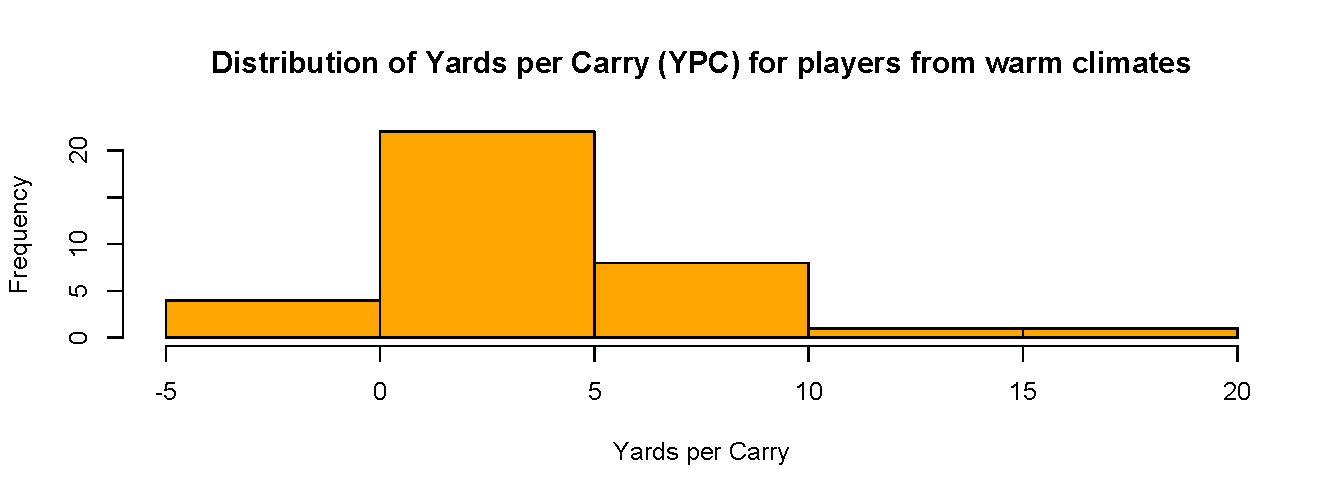
\includegraphics[width=0.8\textwidth]{histW.pdf}
    \caption{Histogram of YPCs for players from warm lifetime climates}
    \label{fig:tikzpgf}
\end{figure}

\noindent After an initial visual check for normality with the histogram, a Shapiro-Wilk test for normality was also used for both groups. For the warm group, the test produced a p-value of 0.0008485 meaning that the data was approximately Normal. The p-value for the cold group was even smaller of 1.914e-07 meaning that data was approximately Normal as well. 

\noindent For a final test of Normality, quantile-quantile plots were developed for the warm and cold groups using the ggplot2 package in R. 

\begin{figure}[htpb]
    \centering
    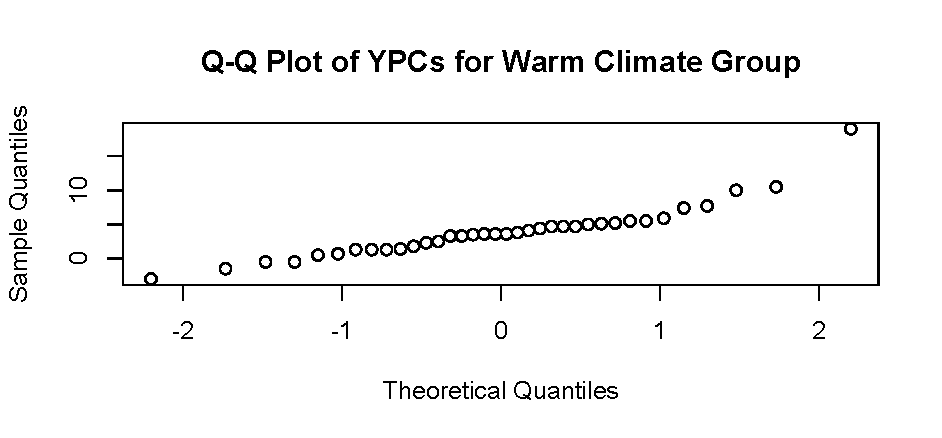
\includegraphics[width=0.8\textwidth]{qqW.pdf}
    \caption{Quantile-Quantile Plot of YPCs for players from warm lifetime climates}
    \label{fig:tikzpgf}
\end{figure}

\begin{figure}[htpb]
    \centering
    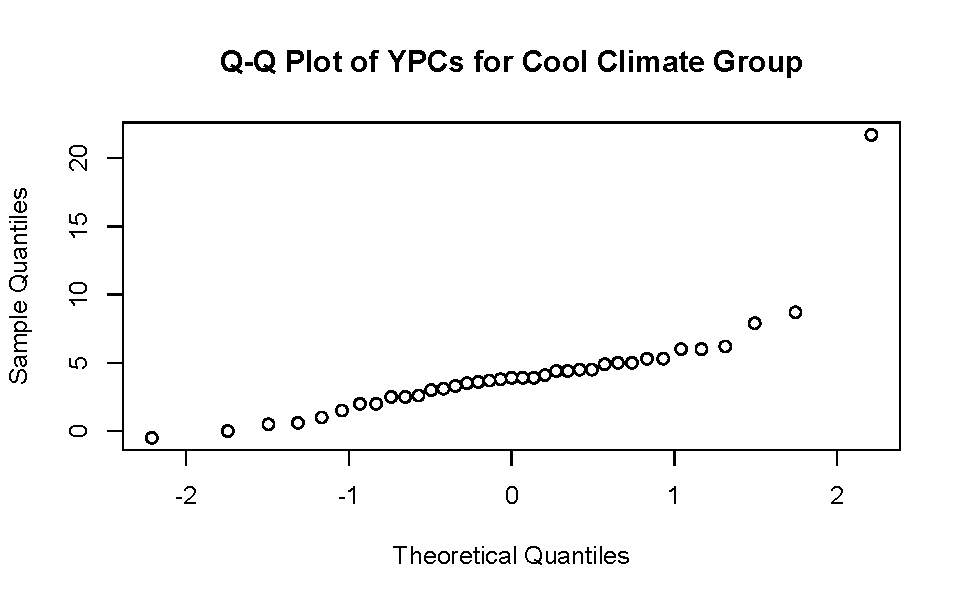
\includegraphics[width=0.8\textwidth]{qqC.pdf}
    \caption{Quantile-Quantile Plot of YPCs for players from cool lifetime climates}
    \label{fig:tikzpgf}
\end{figure}

\noindent Both plots showed that the observed data laid on straight lines, which is indicative of Normally distributed data. \\\\

After, the test for equal variances in R was used and a p-value of 0.6483 was produced, meaning that the null hypothesis (that variances are equal) could not be rejected. Therefore, equal variances was present and we could proceed with the t-test. \\\\

\noindent The null hypothesis of the two sample t-test was that the two sample means were equal. The alternative hypothesis was that the two sample means were not equal. (mean of warm lifetime climate group versus cool lifetime climate group). 

\[H_0: \mu_W = \mu_C\] \[H_a: \mu_W \neq \mu_C\]

\noindent The results of the t-test produced a p-value of 0.7893. The confidence interval for the difference of means was (-1.506269,  1.974587), which includes zero. Since our p-value is much greater than the alpha of 0.05 and zero was included in the confidence interval, we can conclude there is not a significant difference in mean YPC for players from lifetime warm climates and players from lifetime cool climates.\\\\

\section{Discussion}
\noindent There was not a significant difference in mean YPC between the warm lifetime climate group and the cool lifetime climate group. There are many possible explanations for this. This could mean that someone's hometown climate does not affect them as they get older and leave where they come from, meaning that cold weather affects players' performances equally, on average. NFL teams also devote many resources to keeping their players warm when the are off the field. Specialized attire, heated benches, hand warmers, and warm beverages on the sideline all help to alleviate the cold \cite{staywarm}. \\\\

\noindent There are some limitations to this study. Monthly average data is not the most precise weather measurement. To be more precise, future studies could use year-specific weather data for each player; for example, if a player's university was in a warm climate but happened to experience several prolonged cold snaps in a year that a player was there, this could impact a player's adaptation to playing in cold weather. A location with a monthly average of just above 50 degrees will still experience some freezing weather, whereas locations with monthly averages closer to 7 or 80 degrees may rarely experience weather below 60 degrees. The difference in those two climates, for example, would be very large and potentially should not both be grouped together in the warm climate category. Another potential remedy for the generalization of monthly averages would be to select a higher monthly average cut off to maximize the likelihood that the player experienced zero to few days of freezing temperatures. \\\\

\noindent More studies could be used to examine affect of weather on individuals. A study could be used with practice data to see if players on cold weather teams (teams that often see freezing temperatures on their home fields) who had a warm lifetime climate perform worse than other players during their first cold weather season. Using practice data would give more data, thus providing a more reliable and accurate account of a player's performance. Sports physicians, bariatric physicians and evolutionary biologists have published studies in their respective disciplines regarding the role of brown adipose tissue in warming human bodies. Infants have a large percent of brown adipose tissue (BAT). BAT decreases in proportion over the life time, but adults still have this tissue which is critical to body temperature regulation- specifically keeping humans warm. A small number of studies have actually examined how the amount of this tissue can increase when an individual is repeatedly exposed to cold temperatures over a time \cite{coldacclimation}. A study could combine athlete performance with BAT levels of athletes who have spent longer in cooler climates. \\\\

\noindent This study did not double-count individual players. That means that only one game's YPC was used for each player. Single-game statistics may be affected by a variety of factors, such as the opposing team's performance, teammate performance (football carries are impacted by teammates' abilities to protect the RB or other offensive player from a block), as well as chance events that may impact a player's performance (e.g. events in one's personal life). Also, players usually have different amounts of playing times, making comparisons difficult. A new potential study could consider more data points from each player to better control for variation in player performance, as one game is not nearly indicative of a player's true performance. A potential idea would be to calculate an player's average YPC data for one or more seasons and compare this aggregate average to other players' aggregate averages. \\\\

\noindent Lastly, another area of exploration from this paper would be in the field of sports psychology. Players' self-reported confidence to play in cold weather could be compared to their lifetime climate to see if players from warm climates are more likely to report lower confidence in performance in freezing temperatures. 

\newpage
\section{Appendix}

\noindent Table 1 
\begin{center}
\begin{tabular}{|c|c|c|}
\hline
Lifetime Climate Group & Mean & Standard Deviation \\
\hline
Warm & 3.956111 & 3.872995 \\ [1ex]
Cool & 4.17027 & 3.582431 \\ [1ex]
\hline

\end{tabular} 
\end{center}

\begin{figure}[htpb]
    \centering
    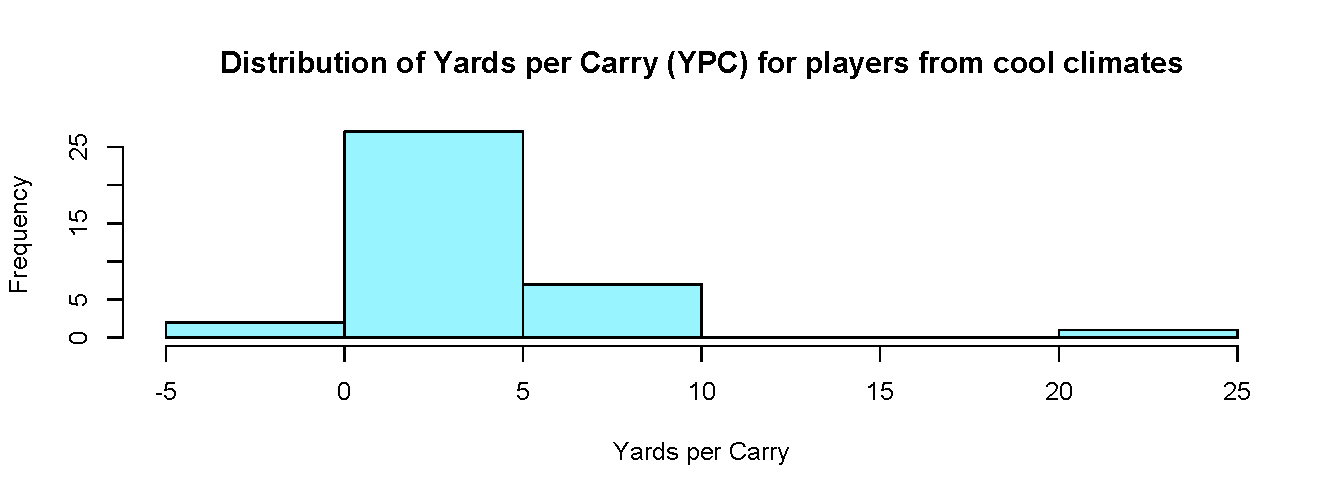
\includegraphics[width=0.8\textwidth]{histC.pdf}
    \caption{Histogram of YPCs for players from cool lifetime climates}
\end{figure}

\begin{figure}[htpb]
    \centering
    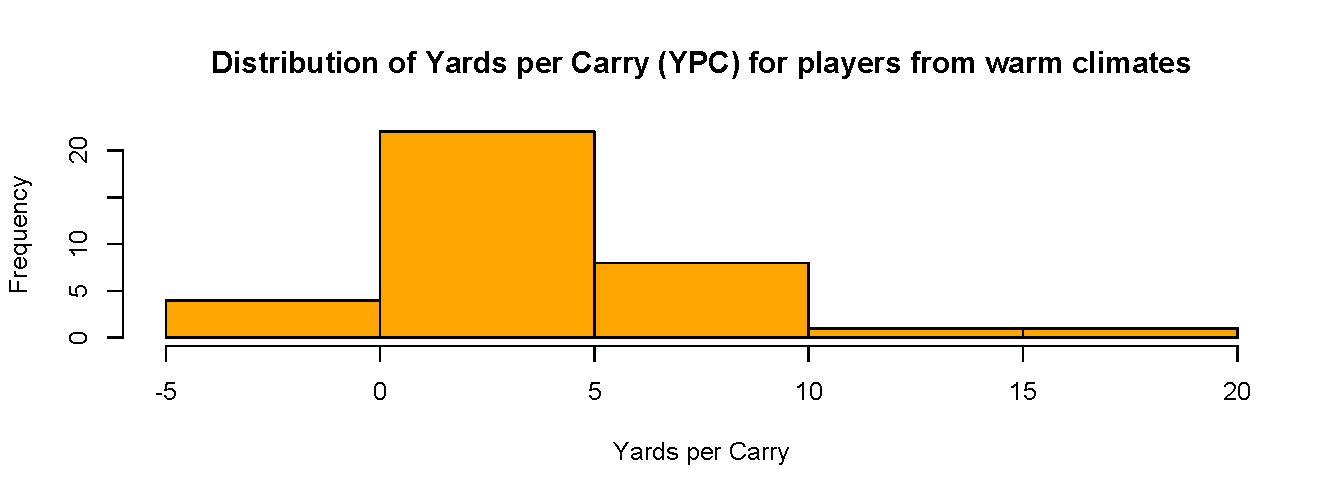
\includegraphics[width=0.8\textwidth]{histW.pdf}
    \caption{Histogram of YPCs for players from warm lifetime climates}
\end{figure}

\begin{figure}[htpb]
    \centering
    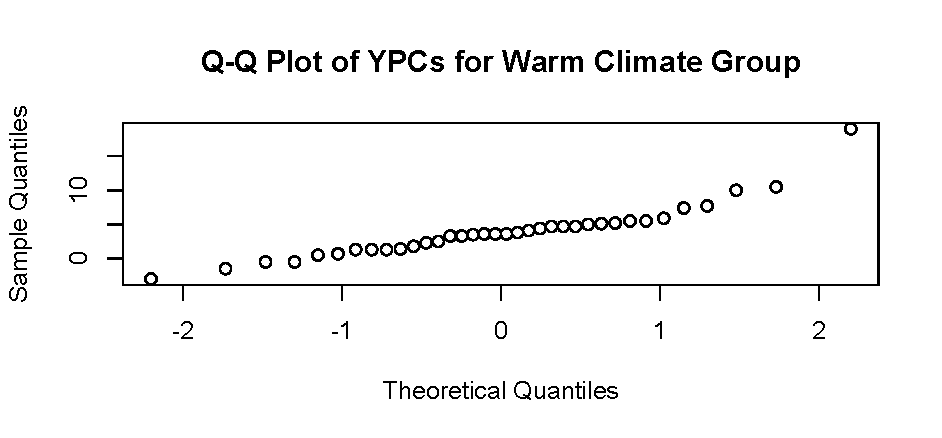
\includegraphics[width=0.8\textwidth]{qqW.pdf}
    \caption{Quantile-Quantile Plot of YPCs for players from warm lifetime climates}
    \label{fig:tikzpgf}
\end{figure}

\begin{figure}[htpb]
    \centering
    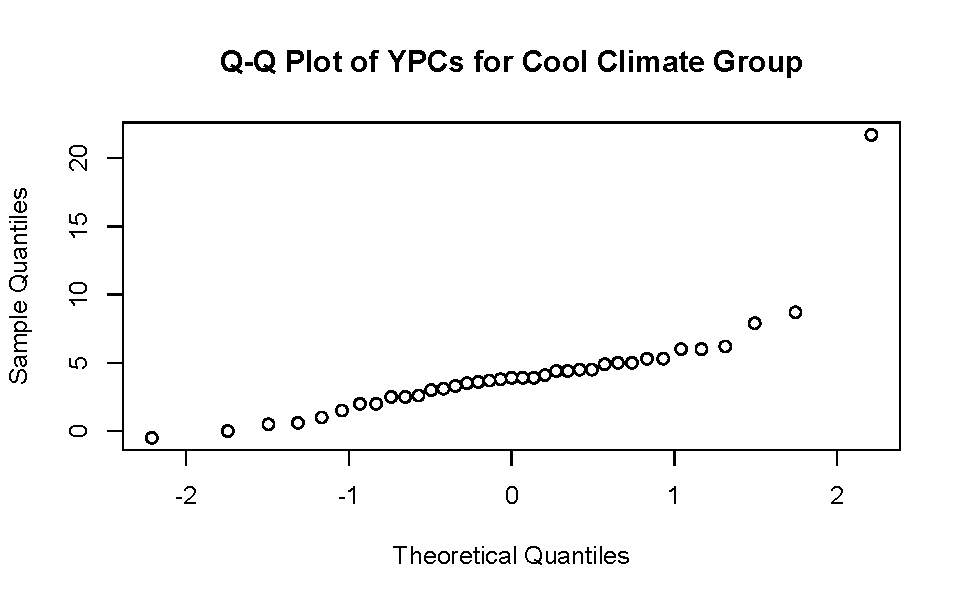
\includegraphics[width=0.8\textwidth]{qqC.pdf}
    \caption{Quantile-Quantile Plot of YPCs for players from cool lifetime climates}
    \label{fig:tikzpgf}
\end{figure}



\newpage
\section{References}
\printbibliography

\end{document}
